\documentclass{scrreprt}
\usepackage[margin=0.7in]{geometry} %réduire marges

\usepackage[french]{babel} %en Français
\usepackage[utf8]{inputenc}
\usepackage[colorlinks=true,urlcolor=blue,linkcolor=blue]{hyperref}
\usepackage[T1]{fontenc}
\usepackage{lmodern}
\usepackage[babel=true]{csquotes}
\usepackage{array}
\usepackage{multicol}
\usepackage{hyperref}

\usepackage[pdftex]{graphicx}
\usepackage{epsfig}


\begin{document}
\pagenumbering{arabic}

\title{iBalezator}
\subtitle{\textit{Cahier des charges}\vspace{-5ex}}
\date{27 février 2015}
\author{Adrien FERREIRA, Alexandra HOSPITAL}
\maketitle
\tableofcontents \newpage


\chapter{Introduction}

\noindent \textbf{Maitrise d’ouvrage :} Thomas Baspeyras, Fabrice Kordon \newline
\noindent \textbf{Maitrise d’oeuvre :} Adrien FERREIRA, Alexandra HOSPITAL\newline

\section{Contexte}


iBalezator est une application pour terminaux sous iOS 8 qui consiste en un jeu de devinette pour mémoriser la disposition des notes sur le manche d’une guitare. Monsieur Baspeyras a réalisé une version web de ce jeu :\newline
\url{http://www.orbite.info/balezator/}\newline
Le but de ce projet est d’adapter ce concept sur petits terminaux sous iOS 8.
L’application s’adresse à des guitaristes débutants sachant lire une partition musicale. Elle propose une aide à la mémorisation des notes sur le manche de la guitare et à la lecture d’une partition.


\section{L’existant}
\subsection{Le site}

Le Balezator en ligne propose plusieurs modes de jeu :
\begin{itemize}

\item Un premier mode permet d'apprendre à identifier une note sur le manche.
On affiche un manche de guitare sur lequel se situe une pastille indiquant la note à trouver.
L'utilisateur dispose d'un clavier sur lequel il peut saisir sa réponse.
Une barre de score est présente pour connaitre le pourcentage de bonnes/mauvaises réponses données.
Il est aussi possible, grâce à des listes déroulantes, de changer l'accordage et de restreindre les questions à un sous-ensemble du manche.\newline

Notre application porte ce mode sur iOS.
L'affichage du manche, de la pastille, du clavier et de la barre de score sont également présents dans notre application.
La restriction des questions est imposée par la portion du manche qu'il est possible d'afficher sur l'écran réduit des terminaux mobiles.
Il n'est pas demandé de proposer un changement d'accordage ou d'instrument.
\medbreak

\item Un deuxième mode permet d'apprendre à identifier une note sur une portée.
Dans la version en ligne, une portée est présentée à l'utilisateur sur laquelle figurent plusieurs notes.
Un fond jaune met en surbrillance la note à deviner sur la portée.
L'utilisateur dispose d'un clavier sur lequel il peut saisir sa réponse. 
Une barre de score est présente pour connaitre le pourcentage de bonnes/mauvaises réponses données.
Il est aussi possible de changer la tonalité, la clé et de restreindre l'exercice à deux ou quatre notes différentes.\newline

Notre application devra porter ce mode sur iOS en remplaçant le mode de saisie.
L'affichage de la portée, des notes et de la barre de score devront être également présents dans notre application.
La différence majeure par rapport au jeu en ligne est que l'utilisateur, pour saisir sa réponse, devra sélectionner la note sur le manche de la guitare et non pas à l'aide du clavier.
Il n'est pas demandé de proposer un changement de tonalité ou une restriction du nombre de notes.
\end{itemize}


\subsection{Première application Balezator}
Une première version du Balezator a été développée. Cette version ne contient qu’un seul mode de jeu : le mode manche/clavier. Notre application devra également contenir ce mode ainsi que le mode portée/manche. Sur un plan plus technique, cette première application est écrite en Objective-C. Notre application devra être développée en Swift. 


\subsection{Applications en concurrence sur l’App-store (veille technologique)}

Parmi les applications étudiées, un sous-ensemble des plus populaires est documenté ci-dessous :

\subsubsection{Guitar Addict} 
Lien : \url{https://itunes.apple.com/us/app/guitar-fretboard-addict/id406919259?mt=8}\\
Prix : 4,99\$
Cette application propose plusieurs modes de jeu. Le manche de la guitare est fixe et l’on doit répondre aux questions en appuyant sur des pastilles positionnées sur une photo de manche.
Selon le mode de jeu, un clavier sur la partie droite est aussi présent. La note à découvrir est également  représentée sur une portée sur la partie inférieure droite de l’écran.
Il est possible de :
\begin{itemize}
\item Choisir l’orientation du manche pour gauchers/droitiers 
\item Notation des notes anglophone ( A, B, C, …) ou françaises (Do, Ré, Mi, …)
\item Le son de la note réponse peut être jouée
\item Notation dièse ou bémol
\item Se focaliser sur une frette, une corde, une tonalité
\end{itemize}

\subsubsection{Trainer HD}
Lien : \url{https://itunes.apple.com/ca/app/trainer-hd-learn-fretboard/id443265532?mt=8}\\
Prix : Gratuit\\
Plusieurs instruments sont proposés dans cette application : ukulélé, banjo, mandoline, guitare 12 cordes.
Le manche est movible par glissé, la note recherchée peut être visualisée sur une portée, un clavier permet de répondre bien qu’il soit aussi possible de répondre directement sur le manche. Un schéma permet également de visualiser les parties du manche sur lesquelles l’utilisateur fait le plus/moins d’erreur en moyenne.
Il est aussi possible de :
\begin{itemize}
\item Choisir l’accordage de la guitare
\item Changer la langue parmi 13 (dont le français)
\item Se focaliser sur une partie du manche
\item Le son de la note réponse peut être jouée 
\end{itemize}

\subsubsection{Guitar Sight Reading Trainer}
Lien :  \url{ https://itunes.apple.com/us/app/guitar-sight-reading-trainer/id390881575?mt=8 }\\
Prix : 2.99\$\\
L’application se focalise uniquement sur les douze premières frettes du manche (il n’est donc pas mobile). Il est cependant possible de réduire les exercices à un sous-ensemble de ces douze frettes. 
Il est possible de :
\begin{itemize}
\item Chercher la note parmi une gamme affichée à l’écran
\item Visualiser son temps de réflexion par groupe de frettes
\item Limiter l'exercice aux notes naturelles, dièse, bémol
\item Changer le mode droitier/gaucher
\item Changer l’accordage parmi 15 disponibles
\end{itemize}

\newpage

\subsubsection{Fret Tester}
Lien :  \url{https://itunes.apple.com/us/app/fret-tester-learn-notes-for/id442144977?mt=8}\\
Prix : 1.99\$\\
Cette application permet le mode de jeu mode Portée/Clavier présent sur le Balézator.
Il est possible de réduire l’exercice avec grande précision en cumulant les critères grâce à une limitation aux seules notes naturelles, bémol, dièses pour un sous-ensemble de cordes, un sous-ensemble de frettes.
Il est possible de :
\begin{itemize}
\item Changer l’accordage
\item S'entraîner sur une guitare douze cordes
\item Afficher les notes sur la portée en clé de sol/fa
\item Visualiser sa progression en pourcentage de bonnes/mauvaises réponses
\item L'exercice à un sous ensemble de la portée
\end{itemize}

\subsubsection{GuitarNotes}
Lien :  \url{https://itunes.apple.com/fr/app/guitarnotes-guitar-fretboard/id492150266?mt=8}\\
Prix : 0.99\$\\
Cette application propose un mode de jeu dans lequel le nom de la note est annoncé avec une voix enregistrée. Il y a également un compteur indiquant le nombre d'occurrences de cette note citée à trouver sur le manche. Les notes tapées sur le manches sont jouées sur les haut-parleurs.
Il est possible de :
\begin{itemize}
\item Réduire l’exercice à un sous-ensemble de cordes/notes
\item Sélectionner la durée de l’exercice
\item Donner une note en fonction de sa position dictée
\item Donner une position en fonction d’une note dictée
\end{itemize}


\chapter{Le produit}
\section{Description de la demande}

Le but du projet est de concevoir une application basée sur le concept du site du Balezator, mais en offrant des modes de jeu adaptés à l’affichage sur terminaux mobiles. Par exemple, sur le site du Balezator, le manche de la guitare est visible entièrement, ce qui n’est pas possible sur terminaux mobiles. Il faut donc adapter l’application.

L’objectif de l’application est de faciliter l’apprentissage des notes du manche de la guitare. L’application se devra d’être disponible hors ligne (sans connexion à Internet), rapide d’utilisation et ergonomique. L’application doit permettre de travailler sur la totalité du manche de la guitare, c’est-à-dire que tout le manche doit être accessible de manière intuitive et ergonomique.

L’application doit fonctionner sous les terminaux ayant une taille d’écran allant de 3,5 pouces à 4,7 pouces et possédant le système iOS 8.


\section{Fonctions du produit}


L’application se présente en mode paysage. Elle propose deux modes de jeu :
\begin{itemize}
\item Portée/manche : L’utilisateur lit des notes présentées sur la portée. Il répond en tapant sur le manche de la guitare qu’il peut faire défiler pour choisir l’emplacement de la note souhaitée. Si l’utilisateur saisit une bonne réponse, la note s’allumera en vert et l’application passera à la note suivante. Sinon, elle s’allumera en rouge et l’utilisateur aura le droit à un nouvel essai jusqu’à ce qu’il trouve la bonne réponse.

\medbreak

\item Manche/clavier : Une question apparaît sur le manche de la guitare sous forme de “pastille” jaune (figure \ref{fig:fig1}) indiquant à l’utilisateur la note à trouver.
A l’aide du clavier présenté dans la partie basse de l’écran, l’utilisateur choisit la note qu’il pense lire.  
Si l’utilisateur saisit une bonne réponse, la “pastille” sur le manche s’allumera en vert (figure \ref{fig:fig2}) et l’application passera à la note suivante. 
Sinon, elle s’allumera en rouge (figure \ref{fig:fig3}) et l’utilisateur aura le droit à un nouvel essai jusqu’à ce qu’il trouve la bonne réponse.
\end{itemize}

\begin{figure}[!ht]
   \centering
   \begin{minipage}[t]{4cm}
      \centering
      
\includegraphics[width=1.5cm]{images/fingering_question.png}
      \caption{Question}
	\label{fig:fig1}
   \end{minipage}
   \begin{minipage}[t]{4cm}
      \centering
      
\includegraphics[width=1.5cm]{images/fingering_good.png}
      \caption{Bonne}
	\label{fig:fig2}
   \end{minipage}
   \begin{minipage}[t]{4cm}
      \centering
      
\includegraphics[width=1.5cm]{images/fingering_bad.png}
      \caption{Mauvaise}
	\label{fig:fig3}
   \end{minipage}
\end{figure}

Score : Une barre de score sera présentée dans la partie haute de l’écran. Elle fera état de la progression de l’utilisateur en affichant une jauge en proportion de bonnes réponses (en vert) et de mauvaises réponses (en rouge).

\chapter{Contraintes}
\section{Contraintes de matériel/logiciel}
Cette application est prévue pour fonctionner sous le système d’exploitation iOS 8, qui inclut les matériels mobiles de la marque Apple.
Le développement est exclusivement effectué sur le logiciel Xcode 6.1 qui permet de réaliser une application fonctionnant sous iOS 8.
Le langage utilisé est Swift avec possibilité d’inclure des portions de code en Objective-C, par exemple, s’il existe des bibliothèques en Objective-C non écrites en Swift.


\section{Contraintes de temps}
Le produit doit être livré avant le 13/05/2015.


\section{Contraintes de programmation}
Le développement doit être effectué en vue de faire évoluer l’application pour y inclure divers modes :
\begin{itemize}
\item multilingue,
\item jeu pour gaucher,
\item jeu pour bassiste,
\end{itemize}
\setlength{\parindent}{1cm}ainsi que sur des terminaux possédant des écrans plus grands (i.e : iPad).


\chapter{Déroulement du projet}

L'équipe de développement est composée d'Adrien FERREIRA et d'Alexandra HOSPITAL.

\section{Organisation}

L’application est développée selon le mode MVC, ce qui implique que chaque nouvelle composante est implémentée par le biais de trois classes : model, view et controller.

\section{Matériel/logiciel utilisés}
Le matériel utilisé pour le développement est un Mac mini sous 10.9.5. Le logiciel utilisé est Xcode 6,1. Les tests seront effectués sur iPod touch MD720NF/A sous iOS 8.1.3.

\section{UML}



\subsection{Cas d’utilisation}

\begin{figure}[!h]
        \centering
        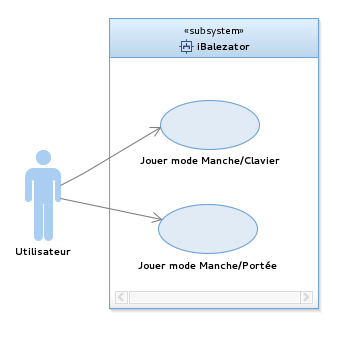
\includegraphics{images/uml_use_case.png}
        \caption{Use case}
        \label{fig:use_case}
\end{figure}


\subsection{Fiche détaillée des cas d’utilisation}

\noindent \emph{Description du cas "Mode Portée/Manche" }
\medbreak
\textbf{Séquencement}\\
Le cas d'utilisation commence quand l'utilisateur lance l'application
\bigbreak

\bigbreak
\textbf{Préconditions}\\
L'utilisateur possède un des terminaux Apple ayant une taille d'écran compris entre 3,5 et 4,7 pouces.\\
La version d'iOS utilisée par l'utilisateur est : iOS 8
\bigbreak


\textbf{Enchaînement nominal}\\
\begin{enumerate}
\item Le sytème affiche une barre de score, une portée et un manche de guitare conformément à la maquette \ref{fig:portee}.
\item Le système popule la portée en fonction de la partie visible du manche. 
\item Le système signe en jaune la première (suivante) note de la portée et un son de guitare fait entendre la note en question.
\item L'utilisateur sélectionne sa réponse sur le manche.
\item Le système, en fonction : 
 \begin{enumerate}
    \item Si la réponse est correcte, fait entendre la note trouvée, la surligne sur la portée, temporise 
    \item Si la réponse est mauvaise, fait entendre la note erronée, la surligne en rouge sur la portée, temporise, retour en SN4
  \end{enumerate}
\item Le système supprime le surlignage de la note.
\item Le système affiche le pourcentage de bonnes/mauvaises réponses en vert/rouge dans la barre de score.
\item retour en SN3
\end{enumerate}
\bigbreak

\textbf{Post-condition}\\
L'utilisateur a pu jouer au iBalézator en mode Portée/Manche.

\bigbreak

\textbf{Enchaînement alternatif}\\
\underline{A1} : Défilement du manche\\
L'enchaînement démarre au point 4 de la séquence nominale :\\
\begin{enumerate}
\item L'utilisateur fait défiler le manche
\item Le système cale la frette la plus proche sur le bord gauche de l'écran
\item Le sytème vide la partition des notes déjà présentes et en affiche de nouvelles en fonction de la partie visible du manche
\item Retour en SN4
\end{enumerate}

\noindent \underline{A2} : Fin de la partition\\
L'enchaînement démarre au point 8 de la séquence nominale :\\
\begin{enumerate}
\item Le sytème vide la partition des notes déjà présentes et en affiche des nouvelles en fonction de la partie visible du manche
\item retour en SN4
\end{enumerate}

\textbf{Enchaînement d'exception}\\
\underline{E1} : Change de mode\\
L'enchaînement peut démarrer au point 4 de la séquence nominale :\\
\begin{enumerate}
\item L'utilisateur touche le bouton de changement de mode
\item Le système demande confirmation à l'utilisateur et change de mode ou non en fonction
\end{enumerate}

\bigbreak
\noindent \emph{Description du cas "Mode Clavier/Manche"}\newline
\medbreak

\textbf{Séquencement}\\
Le système était en mode Portée/Manche et l'utilisateur a appuyé sur le bouton de changement de mode.

\bigbreak
\textbf{Préconditions}\\
L'utilisateur possède un des terminaux Apple ayant une taille d'écran compris entre 3,5 et 4,7 pouces.\\
La version d'iOS utilisée par l'utilisateur est : iOS 8
\bigbreak

\textbf{Enchaînement nominal}\\
\begin{enumerate}
\item Le sytème affiche une barre de score, un manche de guitare et un clavier avec les 12 notes d'une octave conformément à la maquette \ref{fig:clavier}.
\item Le système affiche une pastille "?" sur la partie visible du manche et un son de guitare fait entendre la note en question.
\item L'utilisateur sélectionne sa réponse sur le clavier
\item Le système, en fonction : 
	\begin{enumerate}
	\item Si la réponse est correcte, fait entendre la note trouvée, change la pastille "?" en une pastille <checkmark>, temporise. 
	\item Si la réponse est mauvaise, fait entendre la note erronée, change la pastille "?" en une pastille "x", temporise, change la pastille "x" en pastille "?", retour en SN3
	\end{enumerate}
\item Le système supprime le <checkmark>
\item Le système affiche le pourcentage de bonnes/mauvaises réponse en vert/rouge dans la barre de score
\item retour en SN3
\end{enumerate}
\bigbreak

\textbf{Post-condition}\\
L'utilisateur a pu jouer au iBalézator en mode Clavier/Manche.
\bigbreak
\textbf{Enchaînement alternatif}\\
\underline{A1} : Défilement du manche\\
L'enchaînement démarre au point 3 de la séquence nominale :\\
\begin{enumerate}
\item L'utilisateur fait défiler le manche
\item Le système cale la frette la plus proche sur le bord gauche de l'écran
\item Le système affiche une nouvelle pastille "?" sur la partie visible du manche
\item retour en SN3
\end{enumerate}

\textbf{Enchaînement d'exception}\\
\underline{E1} : Changement de mode\\
L'enchaînement peut démarrer au point 3 de la séquence nominale\\
\begin{enumerate}
\item L'utilisateur touche le bouton de changement de mode
\item Le système demande confirmation à l'utilisateur et change de mode ou non en fonction.
\end{enumerate}

\chapter{Tests de validation}

\section{Scénario logique de l'application}

\begin{figure}[!h]
        \centering
        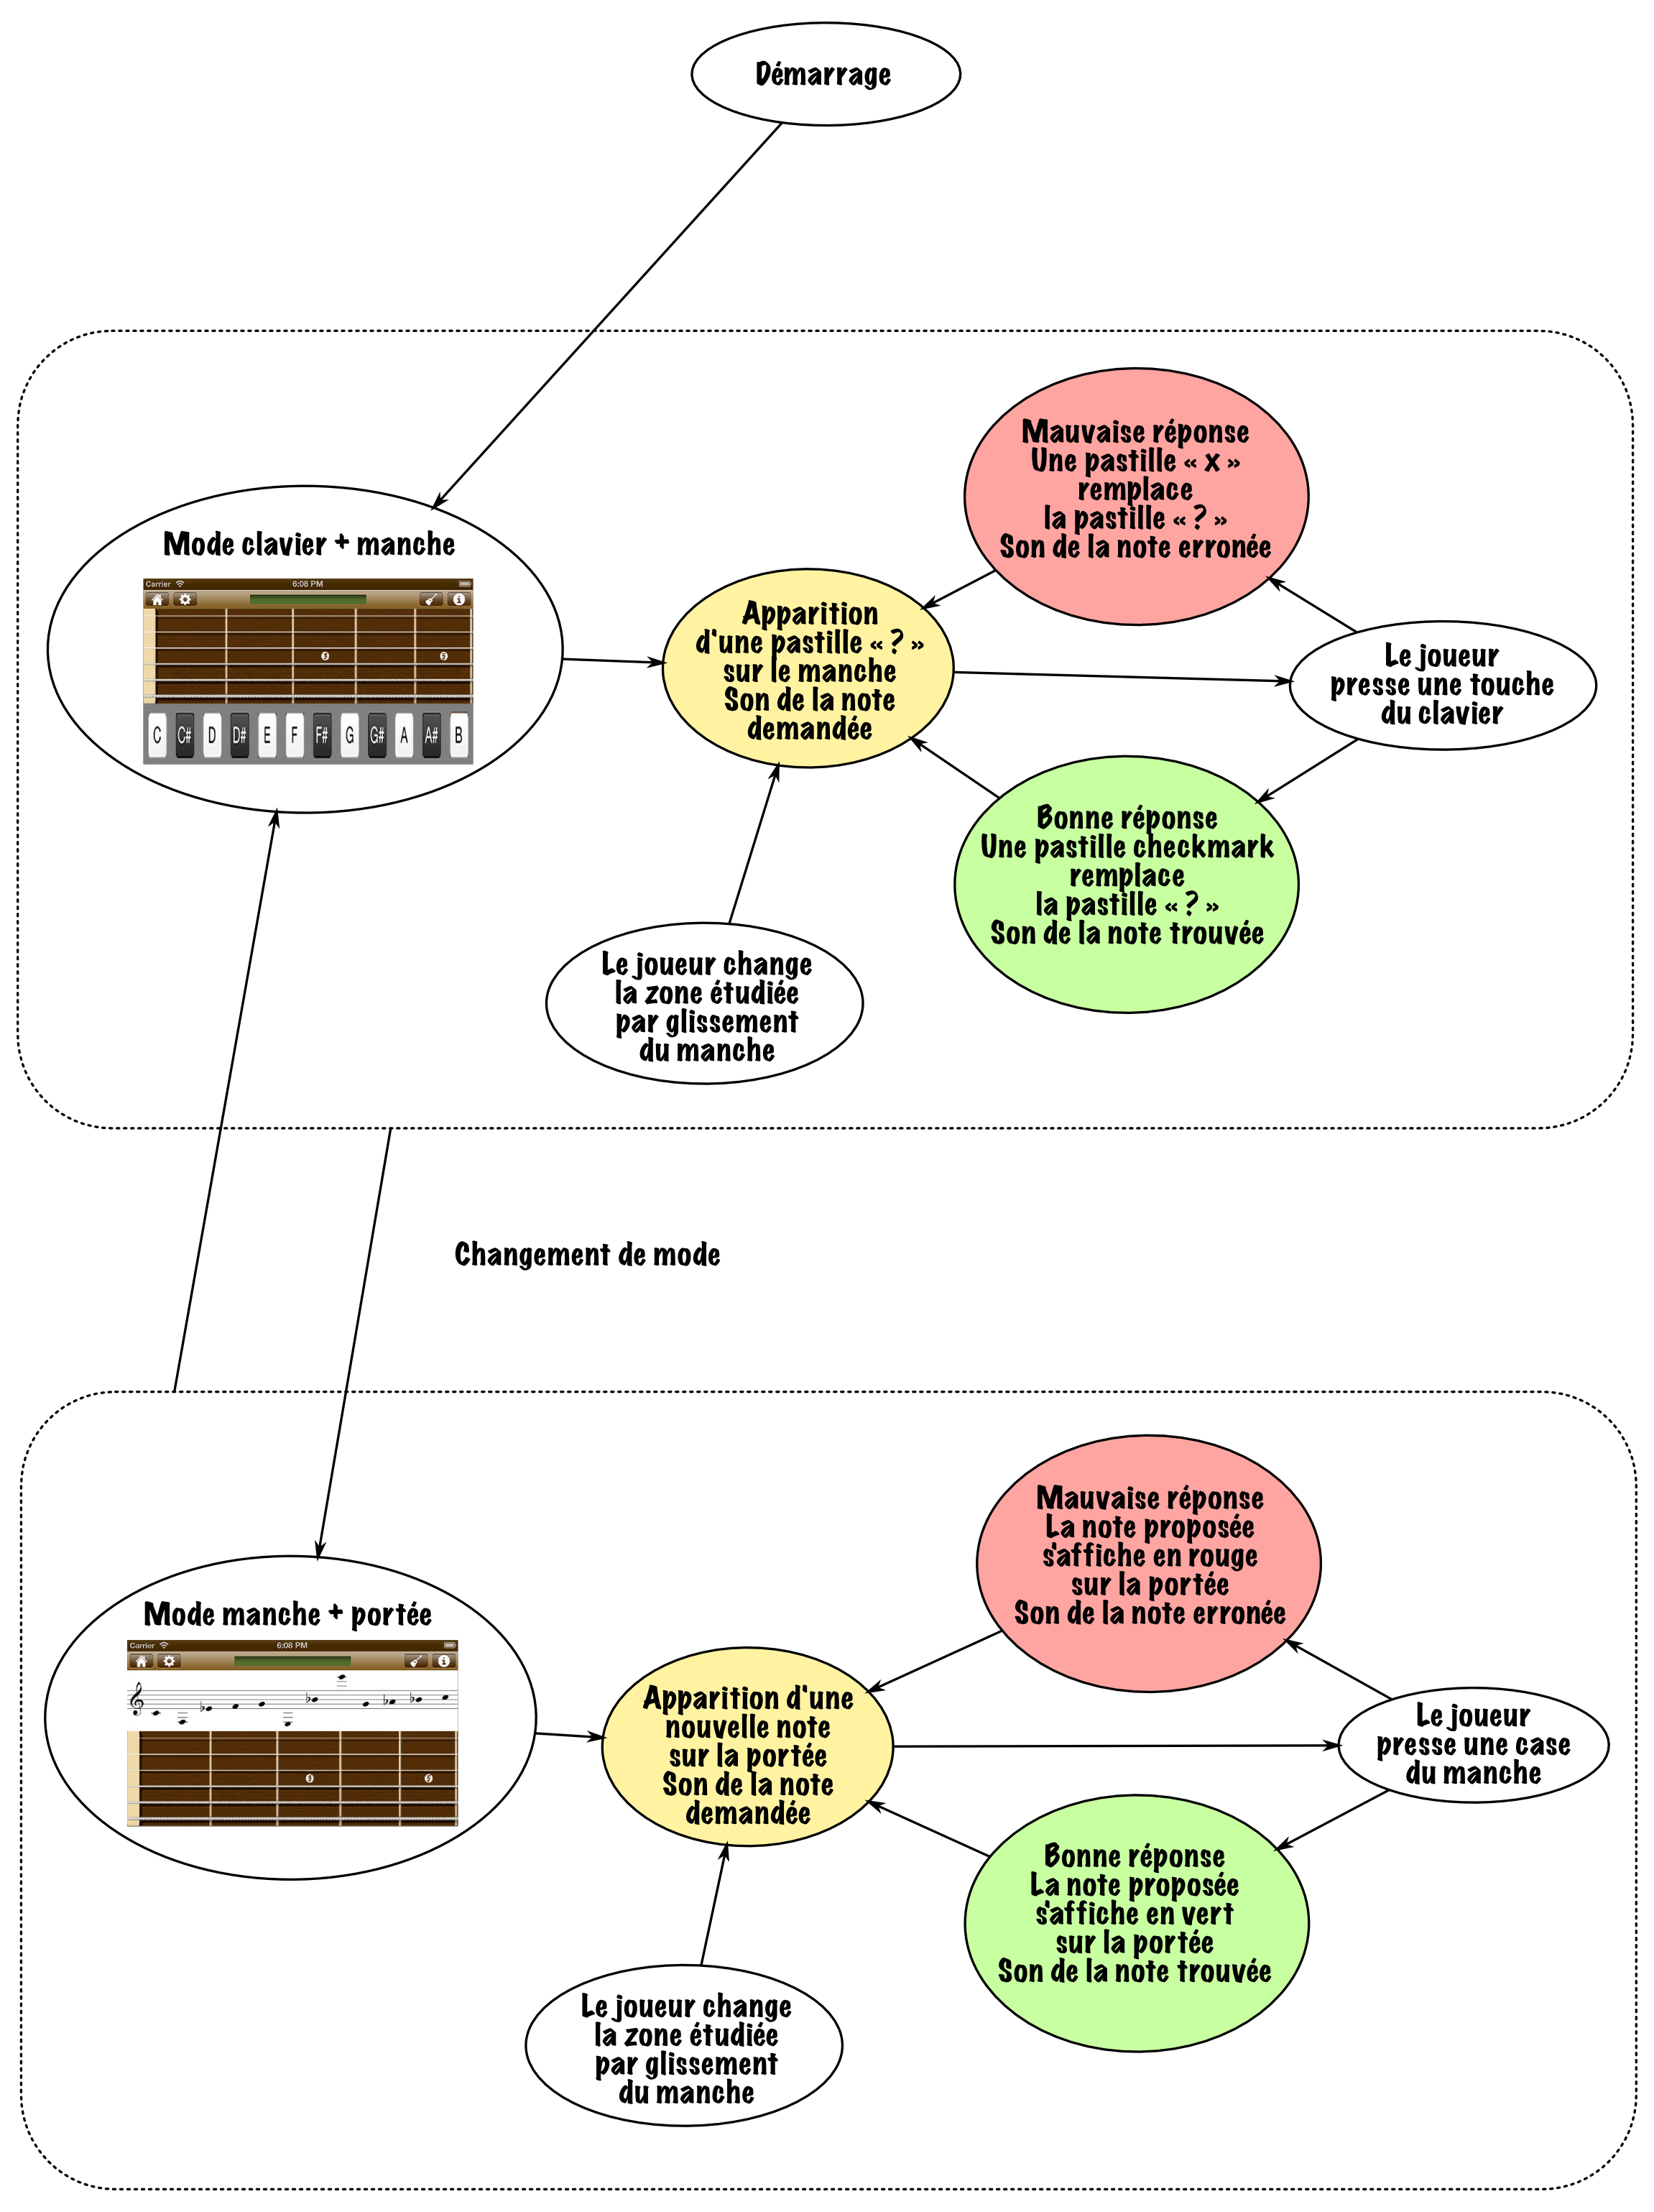
\includegraphics[width=15cm]{images/scenario_balezator.png}
        \caption{Scénario logique de l'application - graphe par Thomas Baspeyras}
        \label{fig:scenarios}
\end{figure}

\section{Maquettes}


\subsection{Mode manche/clavier}

\begin{figure}[!h]
        \centering
        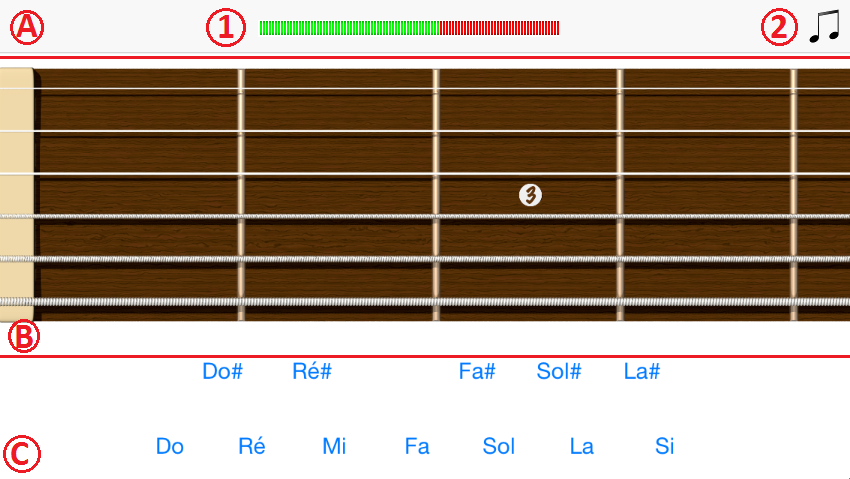
\includegraphics[width=10cm]{images/maquette_usecase/clavier/clavier_zones_ecran.png}
        \caption{Mode manche/clavier}
        \label{fig:clavier}
\end{figure}

Dans ce paragraphe, nous nous référerons à la la figure \ref{fig:clavier} pour les différentes composantes de l’application en mode manche/clavier.\newline
La partie \textbf{A} correspond à la barre de menu contenant la barre de score (élement \textbf{1}) et un bouton de changement de mode 
(élément \textbf{2})\newline
La partie \textbf{B} correspond au manche sur lequel la question est posée.\newline
La partie \textbf{C} correspond au clavier sur lequel l'utilisateur doit taper pour répondre. 
Le clavier se présente comme un clavier de piano : les touches avec une altération dièse (\#) sont noires (non représenté sur la maquette) et se
situent plus haut que les autres touches.
Seules les altérations dièses seront représentées dans cette application. Nous utilisons les notations françaises Do, Do\#, Ré, Ré\#, Mi, Fa, Fa\#, 
Sol, Sol\#, La, La\# et Si.\newline
L'élement \textbf{1} représente la barre de scores de l'utilisateur. Elle contient une proportion de vert à gauche, représentant le pourcentage de
bonnes réponses, 
ainsi qu'une proportion de rouge à droite, représentant le pourcentage de mauvaises réponses.\newline
L'élément \textbf{2} est un bouton permettant à l'utilisateur de changer de mode de jeu. Par exemple, si l'utilisateur se trouve en mode manche/clavier
et qu'il
actionne ce bouton, il sera en mode portée/manche.

\newpage

% ***************** scenario 1 ***************

\subsubsection{Scénario 1}
\bigbreak

\begin{figure}[!ht]
  \begin{minipage}{0.55\linewidth}
    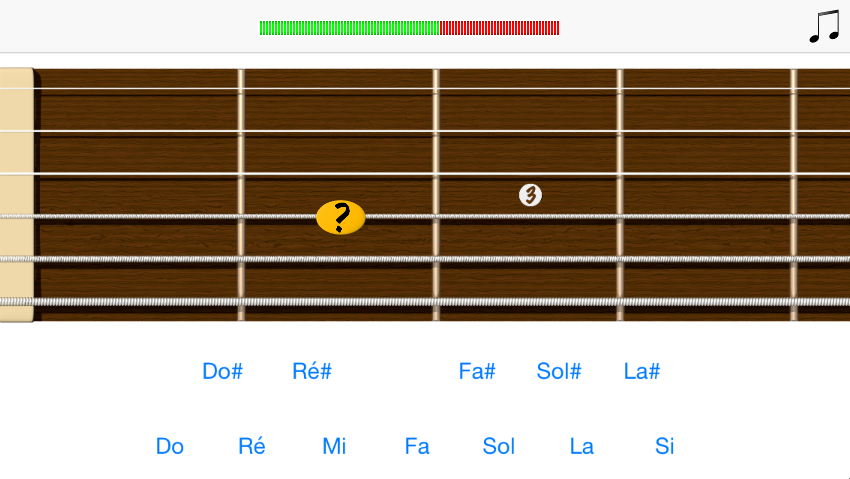
\includegraphics[width=7cm]{images/maquette_usecase/clavier/question.png}
  \end{minipage}\hfill
  \begin{minipage}{0.5\linewidth}
  {Au démarrage de l'application, le système commence en mode manche/clavier. Une question est posée à l'utilisateur. Le son de la note demandée est joué.}
   \end{minipage}
\end{figure}

\bigbreak

\begin{figure}[!ht]
  \begin{minipage}{0.55\linewidth}
    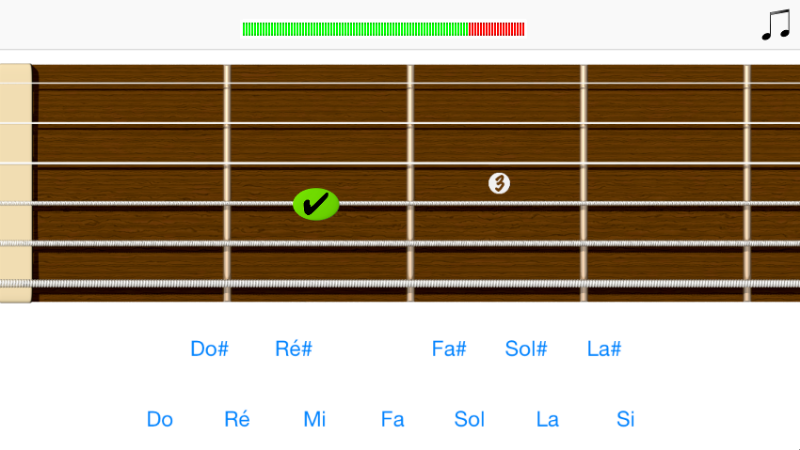
\includegraphics[width=7cm]{images/maquette_usecase/clavier/bonne.png}
  \end{minipage}\hfill
  \begin{minipage}{0.5\linewidth}
  {L'utilisateur a correctement répondu, c'est-à-dire qu'il a tapé sur la bonne touche du clavier (partie \textbf{C}) . La note s'allume en vert avec le son qui lui correspond. La barre de score se met à jour.}
   \end{minipage}
\end{figure}

\bigbreak


\begin{figure}[!ht]
  \begin{minipage}{0.55\linewidth}
    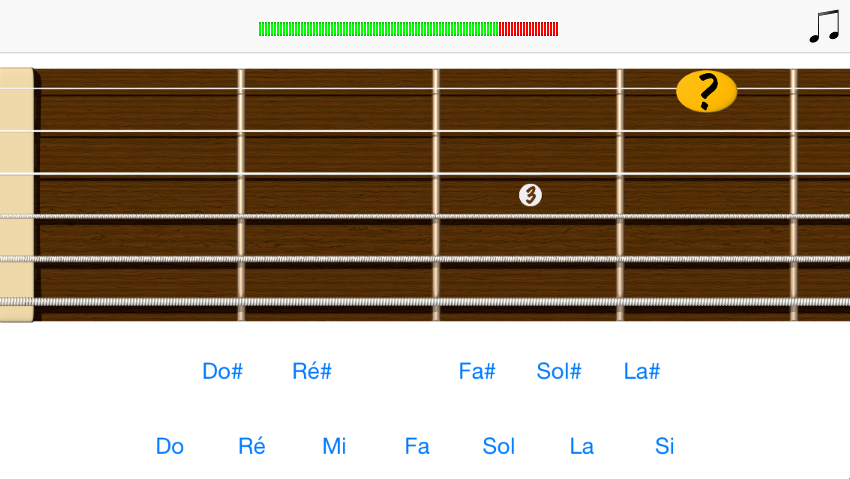
\includegraphics[width=7cm]{images/maquette_usecase/clavier/bonne_reponse_nouvelle_question.png}
  \end{minipage}\hfill
  \begin{minipage}{0.5\linewidth}
  {L'application génère une nouvelle question. L'utilisateur répond à la question comme précédemment.}
   \end{minipage}
\end{figure}

\newpage

% *************** scenario 2 *****************

\subsubsection{Scénario 2}

\begin{figure}[!ht]
  \begin{minipage}{0.55\linewidth}
    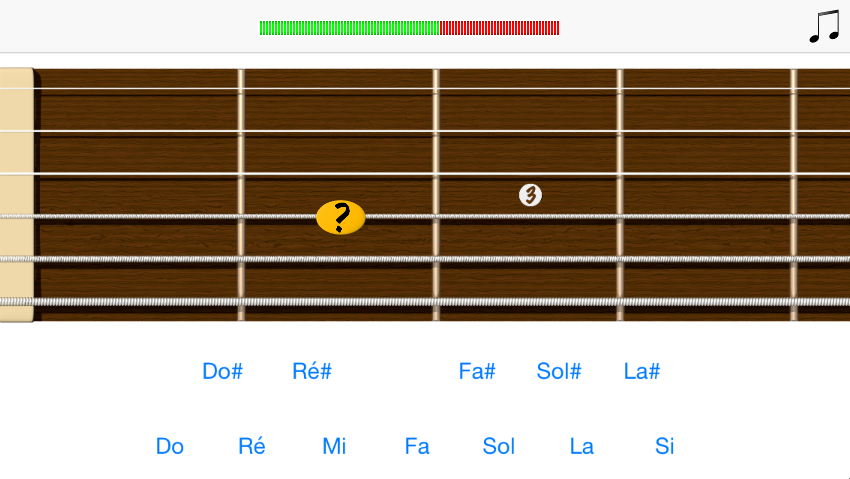
\includegraphics[width=7cm]{images/maquette_usecase/clavier/question.png}
  \end{minipage}\hfill
  \begin{minipage}{0.5\linewidth}
  {Une question est posée à l'utilisateur. Le son de la note demandée est joué.}
   \end{minipage}
\end{figure}

\bigbreak

\begin{figure}[!ht]
  \begin{minipage}{0.55\linewidth}
    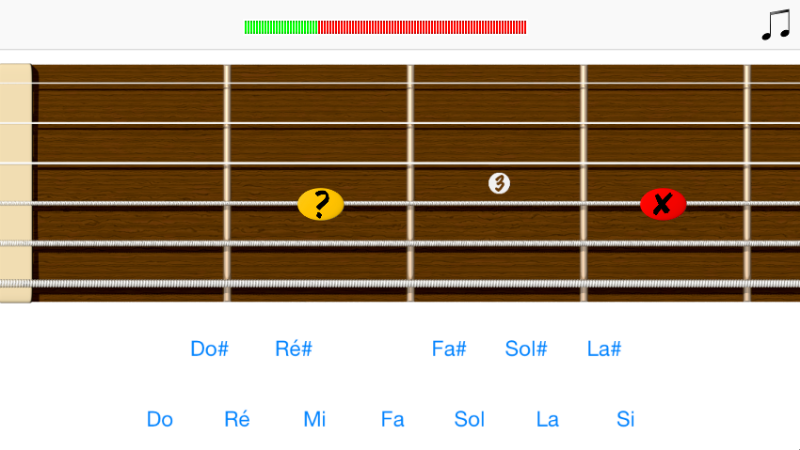
\includegraphics[width=7cm]{images/maquette_usecase/clavier/mauvaise.png}
  \end{minipage}\hfill
 \begin{minipage}{0.5\linewidth}
  {L'utilisateur a entré une mauvaise réponse en tapant sur le clavier (partie \textbf{C}) : la note qu'il a cru lire apparait en rouge sur le manche pour lui donner un indice et la barre de score se met à jour. Le son de la note erronée est joué.}
   \end{minipage}
\end{figure} 

\bigbreak

\begin{figure}[!ht]
  \begin{minipage}{0.55\linewidth}
    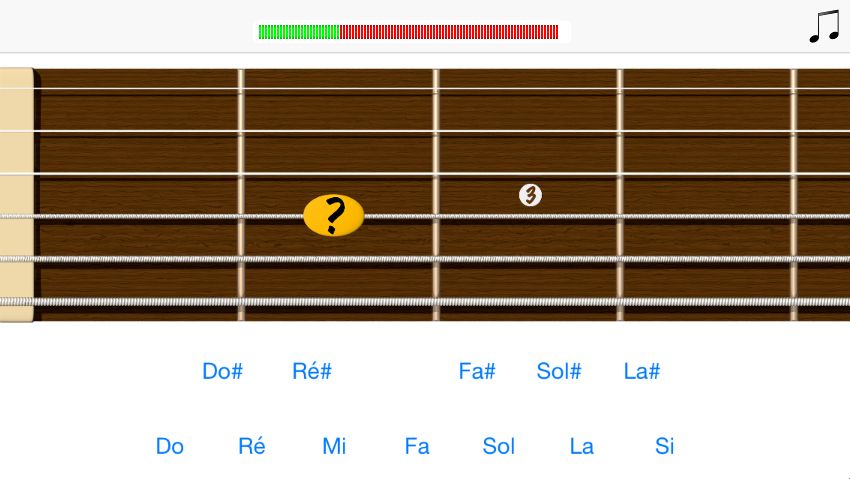
\includegraphics[width=7cm]{images/maquette_usecase/clavier/mauvaise_reponse_nouvel_essai.png}
  \end{minipage}\hfill
  \begin{minipage}{0.5\linewidth}
  {L'application invite l'utilisateur à réessayer. Il répond comme précédemment.}
   \end{minipage}
\end{figure}

\bigbreak

\newpage

% *************** scenario 3 **************

\subsubsection{Scénario 3}

\begin{figure}[!ht]
  \begin{minipage}{0.55\linewidth}
    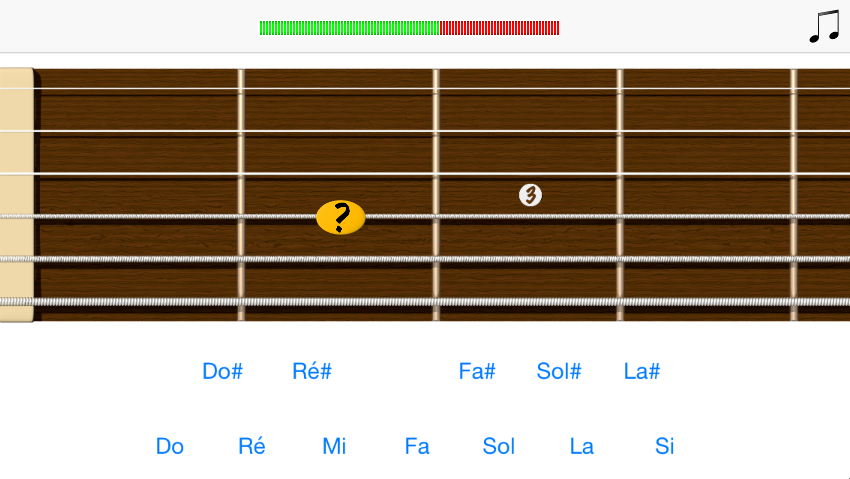
\includegraphics[width=7cm]{images/maquette_usecase/clavier/question.png}
  \end{minipage}\hfill
  \begin{minipage}{0.5\linewidth}
  {Une question est posée à l'utilisateur. Le son de la note demandée est joué.}
   \end{minipage}
\end{figure}

\bigbreak


\begin{figure}[!ht]
  \begin{minipage}{0.55\linewidth}
    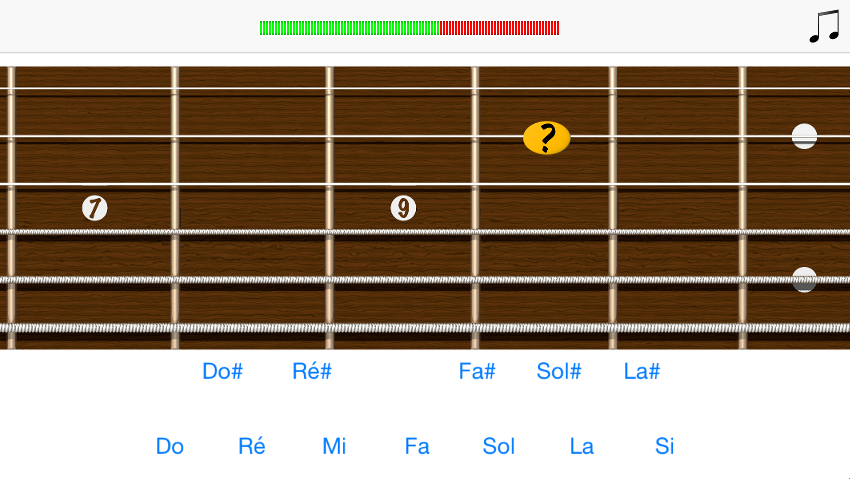
\includegraphics[width=7cm]{images/maquette_usecase/clavier/question_manche_decale.png}
  \end{minipage}\hfill
  \begin{minipage}{0.5\linewidth}
  {L'utilisateur déplace le manche : une nouvelle question est générée dans l'espace visible à l'écran une fois le manche stabilisé (la question précédente est annulée). 
  L'utilisateur répond aux questions de la même façon que dans les scénarios précédents.}
   \end{minipage}
\end{figure}

\bigbreak


\subsubsection{Scénario 4}
\bigbreak

\begin{figure}[!ht]
  \begin{minipage}{0.55\linewidth}
    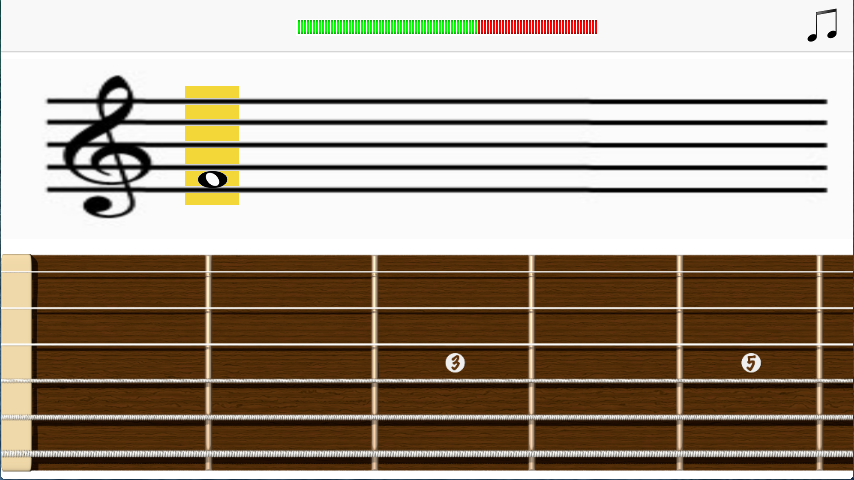
\includegraphics[width=7cm]{images/maquette_usecase/portee/question_une_note_1.png}
  \end{minipage}\hfill
  \begin{minipage}{0.5\linewidth}
  {L'utilisateur change de mode de jeu en appuyant sur l'élément 2 à tout moment : il est désormais en mode portée/manche. Son score portée/manche apparaît.}
   \end{minipage}
\end{figure}


\newpage

\subsection{Mode portée/manche}

\begin{figure}[!h]
        \centering
        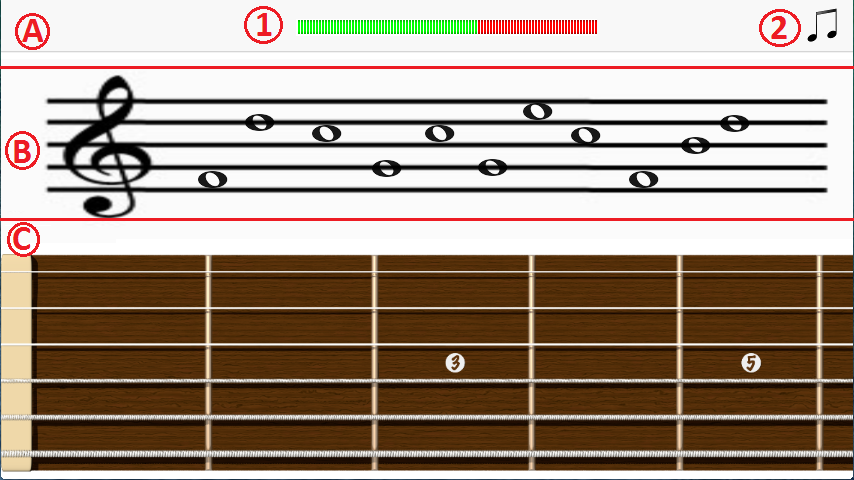
\includegraphics[width=10cm]{images/maquette_usecase/portee/portee_zones_ecran.png}
        \caption{Mode portée/manche}
        \label{fig:portee}
\end{figure}

Dans ce paragraphe, nous nous référerons à la la figure \ref{fig:portee} pour les différentes composantes de l’application en mode portée/manche.\newline
La partie \textbf{A} correspond à la barre de menu contenant la barre de score (élement \textbf{1}) et un bouton de changement de mode (élément 
\textbf{2})\newline
La partie \textbf{B} correspond à la portée sur laquelle l'utilisateur doit lire. Celle-ci ne contient pas d'armure : les altérations sont toutes 
accidentelles. Un signe \enquote{8va} suivi de pointillés surligne les notes aigües pour lesquelles la notation est décalée d'une octave. Les notes sont générées 
au fur et à mesure que l'utilisateur répond.\newline
La partie \textbf{C} correspond au manche de la guitare sur lequel l'utilisateur répond aux questions. Cette partie permet le glissement du manche. Les cordes sont numérotées de 1 à 6, de bas en haut.\newline
L'élement \textbf{1} représente la barre de scores de l'utilisateur. Elle contient une proportion de vert à gauche, représentant le pourcentage de bonnes 
réponses, 
ainsi qu'une proportion de rouge à droite, représentant le pourcentage de mauvaises réponses.\newline
L'élément \textbf{2} est un bouton permettant à l'utilisateur de changer de mode de jeu. Par exemple, si l'utilisateur se trouve en mode portée/manche et 
qu'il actionne ce bouton, il sera en mode manche/clavier.

\newpage


% ***************** scenario 1 ***************

\subsubsection{Scénario 1}

\bigbreak
\begin{figure}[!ht]
  \begin{minipage}{0.55\linewidth}
    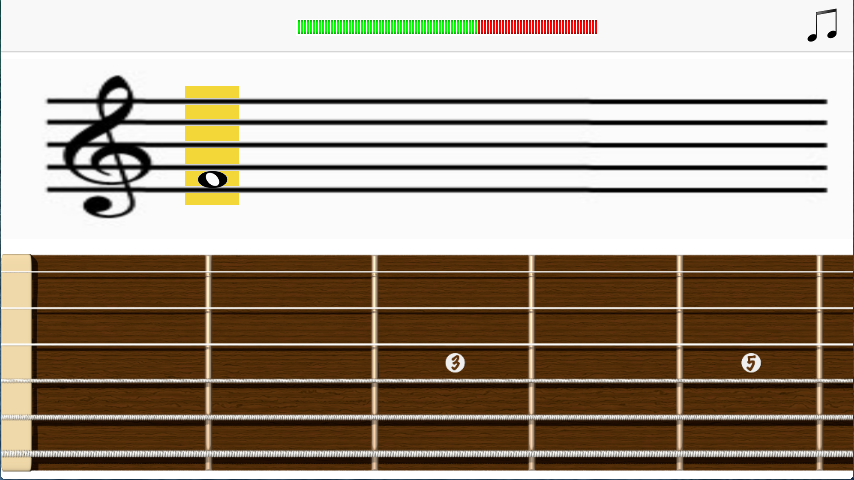
\includegraphics[width=7cm]{images/maquette_usecase/portee/question_une_note_1.png}
  \end{minipage}\hfill
  \begin{minipage}{0.5\linewidth}
  {Une question est posée à l'utilisateur en fonction de la partie visible du manche : la note à trouver est en surbrillance jaune. 
  Le son correspondant à la note est joué.}
   \end{minipage}
\end{figure}

\bigbreak

\begin{figure}[!ht]
  \begin{minipage}{0.55\linewidth}
    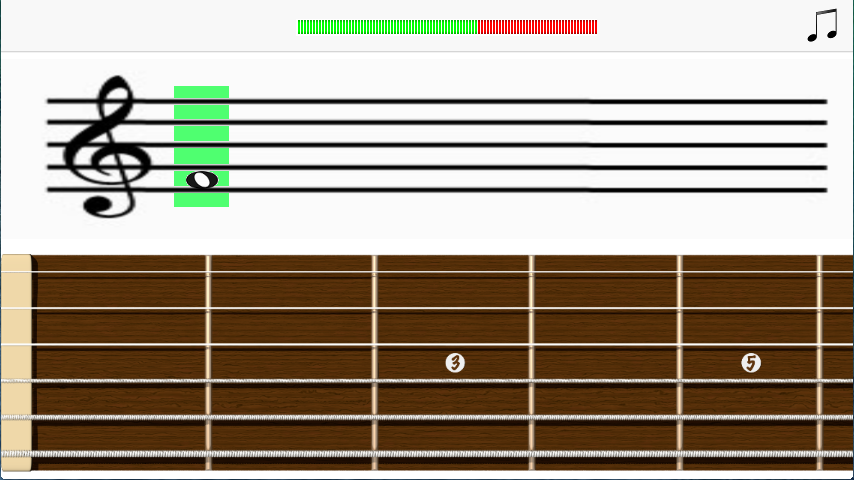
\includegraphics[width=7cm]{images/maquette_usecase/portee/question_une_note_1_vert.png}
  \end{minipage}\hfill
 \begin{minipage}{0.5\linewidth}
  {L'utilisateur a entré une bonne réponse en tapant sur le manche (partie \textbf{B}). La surbrillance de la note devient verte pour le lui indiquer, la barre de score se met à jour. Le son de la note correspondante est joué.}
   \end{minipage}
\end{figure} 

\bigbreak


\begin{figure}[!ht]
  \begin{minipage}{0.55\linewidth}
    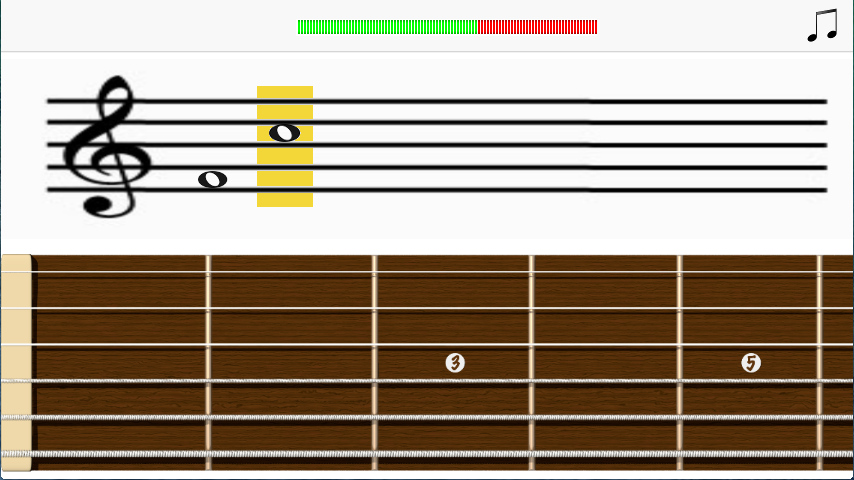
\includegraphics[width=7cm]{images/maquette_usecase/portee/question_une_note_2.png}
  \end{minipage}\hfill
  \begin{minipage}{0.5\linewidth}
  {Une nouvelle question est posée à l'utilisateur. Il répond comme décrit précédemment.}
   \end{minipage}
\end{figure}

\bigbreak

\newpage

% ***************** scenario 2 ***************

\subsubsection{Scénario 2}
\bigbreak


\bigbreak
\begin{figure}[!ht]
  \begin{minipage}{0.55\linewidth}
    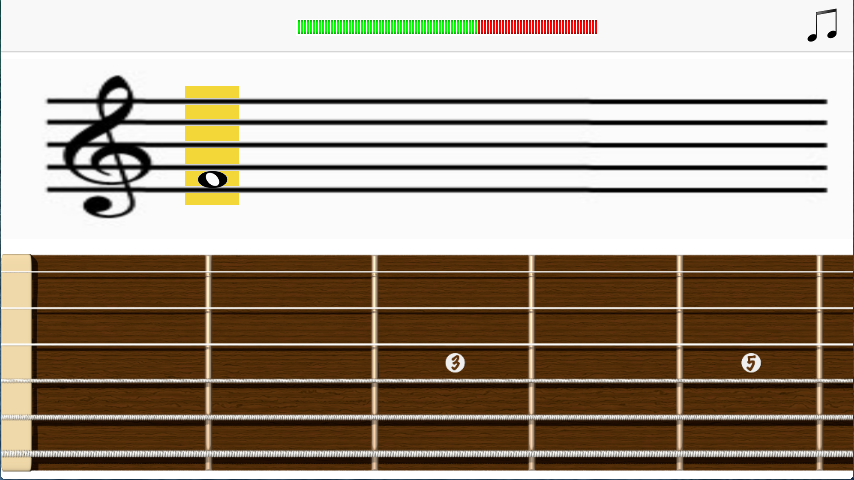
\includegraphics[width=7cm]{images/maquette_usecase/portee/question_une_note_1.png}
  \end{minipage}\hfill
  \begin{minipage}{0.5\linewidth}
  {Une question est posée à l'utilisateur en fonction de la partie visible du manche : la note à trouver est en surbrillance jaune. 
  Le son correspondant à la note demandée est joué.}
   \end{minipage}
\end{figure}



\begin{figure}[!ht]
  \begin{minipage}{0.55\linewidth}
    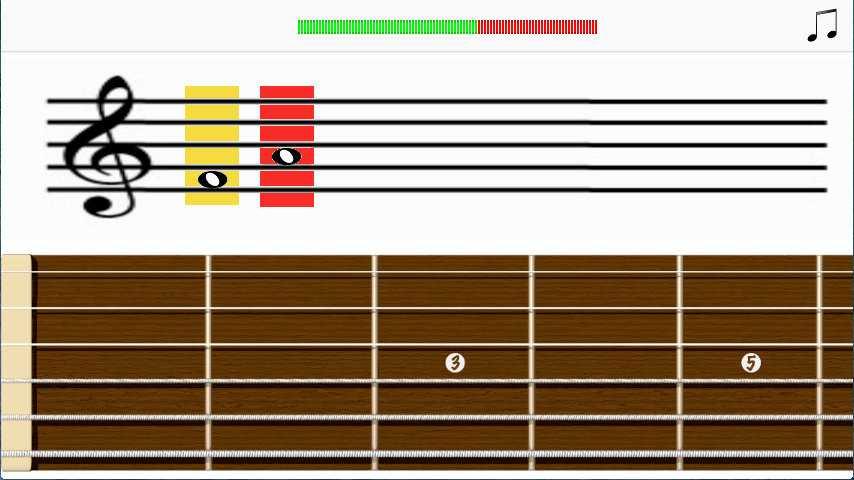
\includegraphics[width=7cm]{images/maquette_usecase/portee/question_mauvaise_reponse.png}
  \end{minipage}\hfill
 \begin{minipage}{0.5\linewidth}
  {L'utilisateur a entré une mauvaise réponse en tapant sur le manche : la note correspondant à sa réponse apparaît sur la portée en surbrillance rouge avec le son de cette note et la barre de score se met à jour. Le son de la note erronée est joué.}
   \end{minipage}
\end{figure}

\bigbreak

\begin{figure}[!ht]
  \begin{minipage}{0.55\linewidth}
    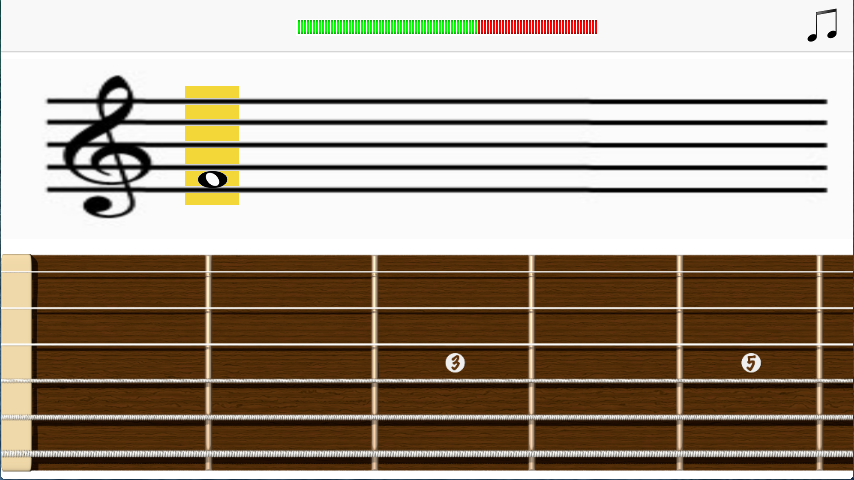
\includegraphics[width=7cm]{images/maquette_usecase/portee/question_une_note_1.png}
  \end{minipage}\hfill
 \begin{minipage}{0.5\linewidth}
  {L'utilisateur est invité à réessayer. L'utilisateur répond à la question comme décrit précédemment.}
   \end{minipage}
\end{figure}

\bigbreak

\newpage

% ***************** scenario 3 ***************

\subsubsection{Scénario 3}
\bigbreak

\bigbreak
\begin{figure}[!ht]
  \begin{minipage}{0.55\linewidth}
    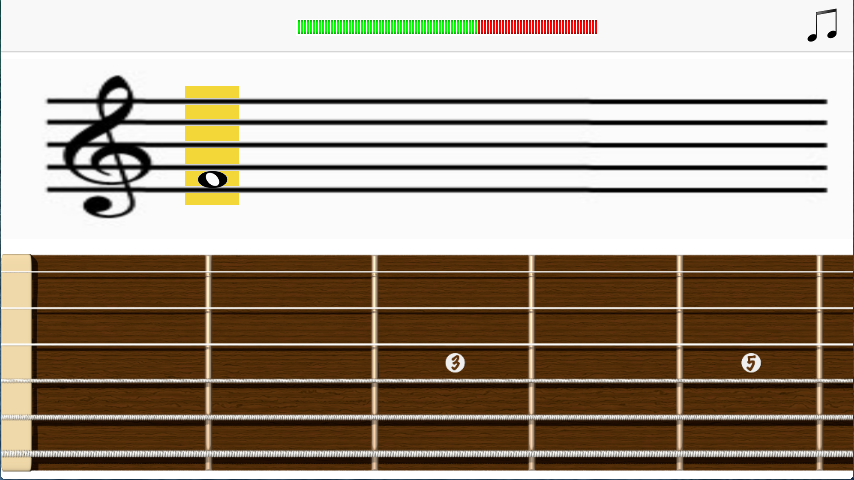
\includegraphics[width=7cm]{images/maquette_usecase/portee/question_une_note_1.png}
  \end{minipage}\hfill
  \begin{minipage}{0.5\linewidth}
  {Une question est posée à l'utilisateur en fonction de la partie visible du manche (partie \textbf{B}) : la note à trouver est en surbrillance jaune. 
  Le son correspondant à la note est joué.}
   \end{minipage}
\end{figure}



\begin{figure}[!ht]
  \begin{minipage}{0.55\linewidth}
    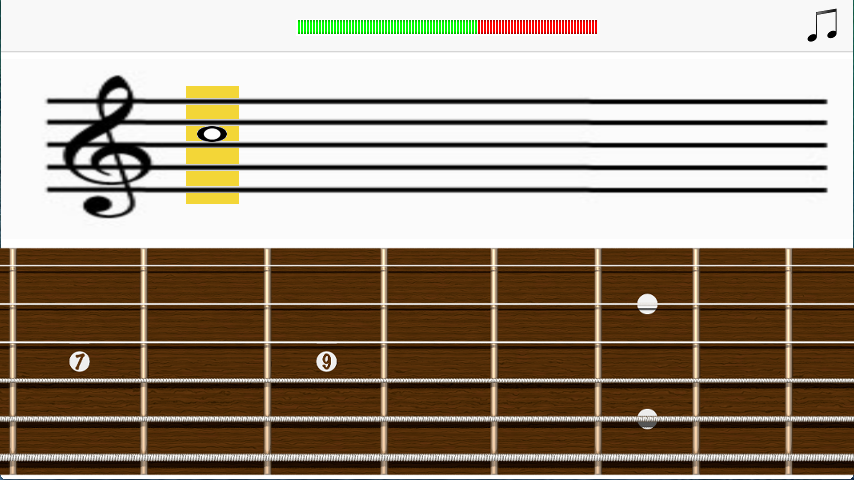
\includegraphics[width=7cm]{images/maquette_usecase/portee/question_changement_manche.png}
  \end{minipage}\hfill
 \begin{minipage}{0.5\linewidth}
  {L'utilisateur change le manche de place en faisant glisser la partie \textbf{B} : une nouvelle question est générée dès que le manche est stabilisé.}
  \end{minipage}
\end{figure}

\bigbreak


\begin{figure}[!ht]
  \begin{minipage}{0.55\linewidth}
    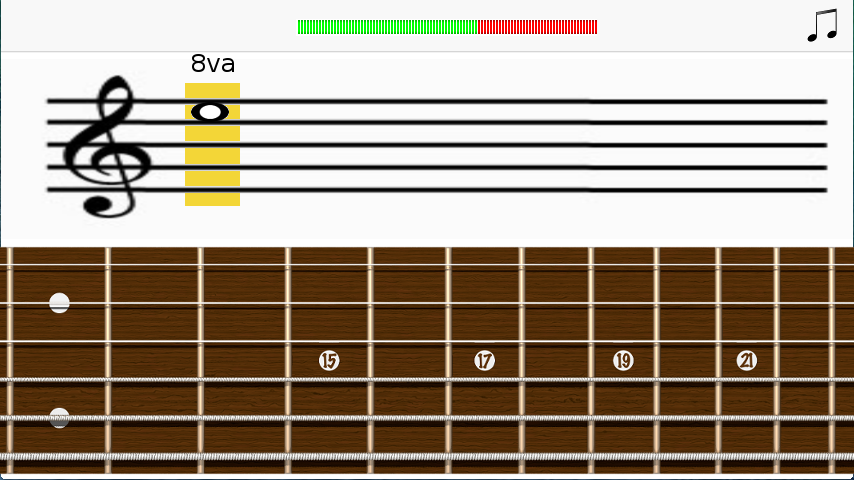
\includegraphics[width=7cm]{images/maquette_usecase/portee/8va.png}
  \end{minipage}\hfill
 \begin{minipage}{0.5\linewidth}
  {Si le manche dépasse la 12ème case et que la question est une note sur les cordes 1, 2 et 3, l'étiquette \enquote{8va} apparaît en haut de la portée.}
   \end{minipage}
\end{figure}

\bigbreak

% ***************** scenario 4 ***************

\subsubsection{Scénario 4}
\bigbreak


\begin{figure}[!ht]
  \begin{minipage}{0.55\linewidth}
    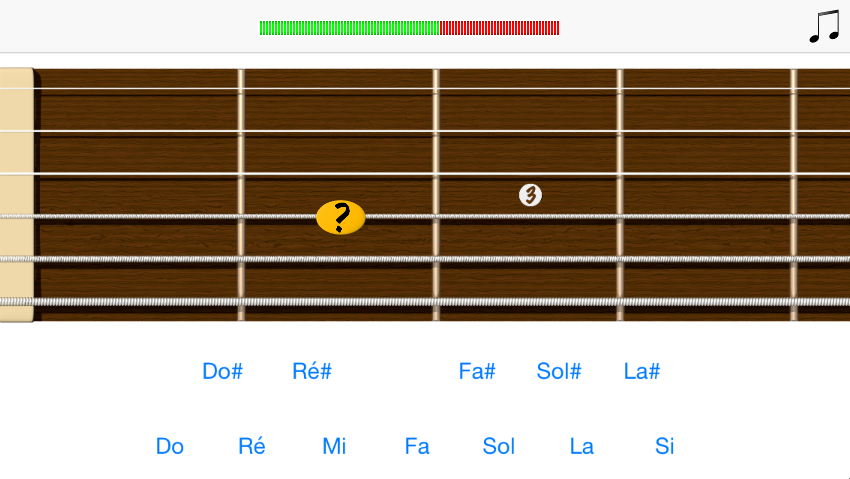
\includegraphics[width=7cm]{images/maquette_usecase/clavier/question.png}
  \end{minipage}\hfill
 \begin{minipage}{0.5\linewidth}
  {L'utilisateur change de mode de jeu en tapant sur l'élément \textbf{2} à n'importe quel moment : il est désormais en mode manche/clavier. Son score manche/clavier apparaît.}
   \end{minipage}
\end{figure}

\bigbreak

\newpage

% ***************** scenario 5 ***************

\subsubsection{Scénario 5}
\bigbreak

\begin{figure}[!ht]
  \begin{minipage}{0.55\linewidth}
    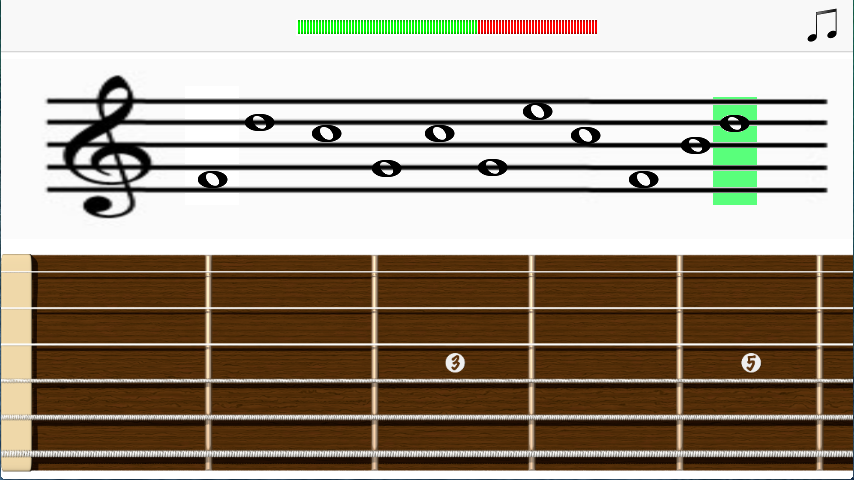
\includegraphics[width=7cm]{images/maquette_usecase/portee/question_portee_remplie.png}
  \end{minipage}\hfill
 \begin{minipage}{0.5\linewidth}
  {Les notes sont générées au fur et à mesure des bonnes réponses de l'utilisateur et s'ajoutent sur la portée jusqu'à la remplir. Sur cet exemple, l'utilisateur a bien répondu à 11 questions.}
   \end{minipage}
\end{figure}

\bigbreak

\begin{figure}[!ht]
  \begin{minipage}{0.55\linewidth}
    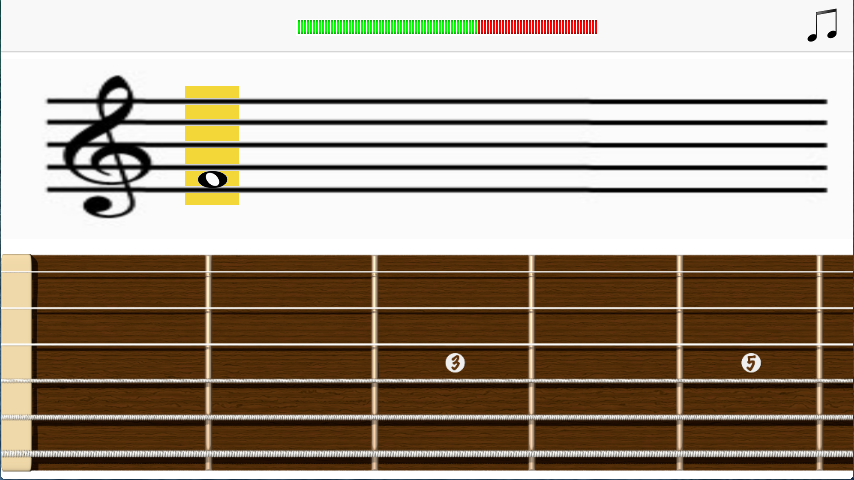
\includegraphics[width=7cm]{images/maquette_usecase/portee/question_une_note_1.png}
  \end{minipage}\hfill
 \begin{minipage}{0.5\linewidth}
  {Lorsque la portée est entièrement remplie, elle est vidée et les notes sont générées comme décrit précédemment.}
   \end{minipage}
\end{figure}

\bigbreak




\section{Remarque}

L'idée originelle du client était d'implémenter le changement de mode de jeu par glissement vertical sur l'écran. 
Cependant cette solution n'est pas obligatoirement celle qui sera implémentée, sous réserve de sa faisabilité et de son utilisabilité.

\end{document}
